\chapter{\chai}
This chapter starts with an introduction to {\mocha } \cite{Mo98}, on
which \chai \ is built. It is then is followed by a tutorial on
modelling and verification using {\chai}. Towards the end of the
chapter the details of {\im}, their implementation, and their usage are
presented.

\section{The Starting Point- \mocha} \chai \ is based on {\mocha },
it extends the functionality of \mocha \ and adds an input
language to suit interfaces.

\mocha \ is an interactive environment for modular verification of
%<<<<<<< chai.tex
%heterogeneous systems of digital components, including those that
%are synchronous or asynchronous, speed-independent or real-time,
%and finite or infinite state. {\mocha } relies on the modelling
%framework of reactive modules unlike traditional use of state
%transition graphs. Its input language is machine readable variant
%of reactive modules. In \chai \ we extend \rm \ to interface
%modules as explained in next chapter.
%=======
heterogeneous systems of digital components.  \mocha \ relies on the
modelling framework of reactive modules. Its input language is a machine
readable variant of reactive modules. In \chai \ we extend \rm \ to
interface modules as explained in the next chapter.
%>>>>>>> 1.19

%\section{Mocha}
%Some lines on mocha implementation


%This section describes Mocha in summary detail.
\mocha \ supports the following functionalities \cite{mochaman}:
\begin{itemize}
\item \textbf{System specification} in the language of Reactive
Modules. Reactive Modules allow the formal specification of
heterogeneous systems with synchronous, asynchronous, and
real-time components. Reactive Modules support modular and
hierarchical structuring and reasoning principles.

\item \textbf{System execution} by randomized, user-guided, or
mixed-mode trace generation. In mixed-mode trace generation, the
user plays a game against \mocha \ and guides the execution of
some modules, while \mocha \ controls the execution of other
modules.

\item \textbf{Requirement specification} in Alternating Temporal
Logic \cite{ATL}. The logic ATL allows the formal specification of
requirements that refer to collaborative as well as adversarial
relationships between modules. The popular logic CTL
(Computational Tree Logic) \cite{ATL} is a sublanguage of ATL.

\item \textbf{Requirement verification} by ATL model checking. The
symbolic model checker in both implementations is based on BDD
engines developed by the UC Berkeley VIS project \cite{VIS96}. For
invariant checking, \mocha \ supports both symbolic and
enumerative search.

\item \textbf{Implementation verification} by checking trace
containment between implementation and specification modules.
\mocha \ supports containment checking if the specification module
has no hidden state, and simulation checking otherwise. For
decomposing proofs, \mocha \ supports an assume-guarantee
principle.

\item \textbf{Reachability analysis} of real-time systems.
\end{itemize}

In \mocha\ the basic structuring units, or the molecules of a
system, are {\em reactive modules} \cite{RM96journal}. The modules have
a well-defined interface given by a set of \emph{external (or
input)} variables and a set of {\em interface (or output)}
variables. A module may also have a set of {\em private}
variables. All variables are typed, and \mocha \ supports a
standard set of finite and infinite types, such as boolean and
integers. A module is built from \emph{atoms}, each grouping
together a set of \emph{controlled} (interface or private)
variables with exclusive updating rights.

\emph{Updating} is defined by two nondeterministic guarded
commands: an \emph{initialization} command and an \emph{update}
command. These commands decide the new value of the controlled
variable by picking up the guarded commands non-deterministically.
In these commands unprimed variables, such as $x$, refer to the
old value of the corresponding variable, and primed variables,
such as $x'$, refer to the new value of the corresponding
variable.  An atom is said to \emph{await} another atom if its
initialization or update commands refer to primed variables that
are controlled by the other atom.

The variables change their values over time in a sequence of
\emph{rounds}. The first round consists of the execution of the
initialization command of each atom, and the subsequent rounds
consist of the execution of the update command of each atom,  in
an order consistent with the await dependencies. A round of an
atom is therefore a \emph{subround} of the module. If no guard of
the update command is enabled, then the atom idles,
i.e., the values of the variables do not change.  %If the update
%command of an atom has a branch with a true guard and no updating
%action, then it may at any time either take a transition or idle.
%Such an atom is called \emph{lazy}, and is useful for modelling
%asynchronous interaction.
%
%%%Use a better example ?
%For example, consider the specification of a village telephone
%system that contains four telephones. The specification consists
%of two modules: the first one models the environment, i.e., the
%users, and the second one models the system. A phone is either
%on-hook or off-hook, and the module {\tt UserSpec}
%nondeterministically toggles at most one telephone between on-hook
%and off-hook.
%\begin{example}{}
%\begin{verbatim}
%type hookType is {on, off} module UserSpec is
%  interface h1,h2,h3,h4: hookType;
%lazy atom ToggleHook
%  controls h1,h2,h3,h4
%  reads h1,h2,h3,h4
%  init
%    [] true -> h1' := on; h2' := on; ...
%  update
%    [] h1 = on -> h1' := off;
%    [] h1 = off -> h1' := on;
%    ...
%  endatom
%endmodule
%\end{verbatim}
%\end{example}

Modules can be \emph{composed} if they have disjoint sets of
interface variables, and their union of atom sets does not contain
a circular await dependency. Given a specification {\tt
SystemSpec} of a system and model of user behavior as {\tt
UserSpec}, specification module {\tt Spec} is defined as:
\vspace*{-2ex}
\begin{footnotesize}
\begin{verbatim}
module Spec is UserSpec || SystemSpec
\end{verbatim}
\end{footnotesize}
\vspace*{-2ex} For encapsulation \rem{} allows the {\em hiding} of
interface variables, and for instantiation it allows the {\em
renaming} of interface and external variables. Hiding and parallel
composition permit hierarchical descriptions of complex systems.

\section{Tutorial Introduction to \chai}
%This section starts with a quick taste of chai.
Chai will be available for free public download from
\cite{getchai}. It requires the GLU BDD package and Tcl7.2. The
installation instructions and relevant notes are available at
\cite{getchai}.

\subsection{Modelling with \chai}
Consider modelling the 2-bit down counter shown in Figure
\ref{fig:downcounter} as an interface module. The counter counts
from 3 to 0 on its normal run. Whenever the reset is high the
counter resets itself to start down counting from 3. Thus we have
the input, reset and outputs, counting bits $b0$ and $b1$.

To model this downcounter as an interface we should first
understand the input assumption and output guarantee of the
system. In case of the downcounter, the input assumption is fairly
trivial, the input \emph{reset} can be either 1 or 0. So we choose
it to be non- deterministic denoted as \texttt{nondet}. The output
guarantee is that counter counts from $3 \rightarrow 2 \rightarrow
1 \rightarrow 0 \rightarrow 3$ when it is not reset and on being
reset starts counting from 3. We represent this as guarded
commands. If the state of counter (reset,b1,b0) is (0,1,0) then in
the next state it should move to zero if the reset stays low i.e
(0,0,0) low so we have a guarded command as shown below. Note that
the control variables (b1, b0) take the values (false, true) only
if the guard on left of right arrow is true.
\begin{verbatim}
       [] ~reset &  b1 & ~b0 -> b1' := false; b0' := true
\end{verbatim}

Figure \ref{fig:modeldowncounter} shows the interface module for
the down counter shown in Figure \ref{fig:downcounter}.

\begin{figure}[htbp]
\centering
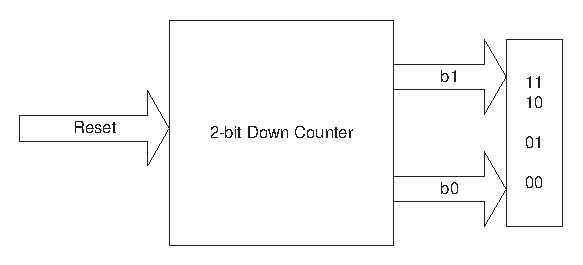
\includegraphics[width=4in]{figs/downcounter}
\caption{A 2-bit Down Counter}
\label{fig:downcounter}
\end{figure}

\begin{figure}[h]
\centering
\input{egs/downcounter.intf}
\caption{A 2-bit Down Counter Modelled As An Interface Module}
\label{fig:modeldowncounter}
\end{figure}

\subsection{Running \chai}
All the interface module definitions have to be entered into a
single file named typically with the suffix .intf; in our case,
(say) this file is downcounter.intf (Figure
\ref{fig:modeldowncounter}). \chai \ is invoked by typing {\tt
chai} at the shell prompt.

\begin{verbatim}
kala 6> chai
Welcome to CHAI 1.0
Please report any problems to dvl@cse.ucsc.edu
chai 1.0 >
\end{verbatim}

\noindent The interface is read and parsed with the {\tt
read\_intf} command. As shown below \chai \  displays the names of
the modules that were successfully parsed. In the case of a parse
error, an appropriate message is displayed.

\begin{verbatim}
kala 68> chai
Welcome to CHAI 1.0
Please report any problems to dvl@cse.ucsc.edu
chai 1.0 > read_intf downcounter.intf
...
DEBUG Interface Created: downcounter
chai 1.0 >
\end{verbatim}

\chai \ provides many methods and tools for verifying the
correctness of a design: execution (i.e., simulation), invariant
checking, refinement checking, ATL model checking, interface
composition. Interface composition being the distinguishing
feature of \chai \ we detail it here, the rest of the features are
described in \cite{mochaman}.

The command for interface composition is {\tt compose\_intf}.
\begin{verbatim}
chai 1.0 > compose_intf
Usage: compose_intf <outIntf> <Intf1> <Intf2>
\end{verbatim}

\noindent It checks if the interfaces {\tt Intf1} and {\tt Intf2}
can be composed as a new interface {\tt outIntf}. When we run this
command on interface downcounter (Figure \ref{fig:downcounter} )
and a dual output gate (Figure \ref{fig:gate}).
\begin{figure}[h]
\centering
\input{egs/gate.intf}
\caption{A Simple Gate} \label{fig:gate}
\end{figure}
The composition gives a compatible interface as following \chai \
session shows.
\begin{verbatim}
chai 1.0 > read_intf downcounter.intf
...
chai 1.0 > read_intf gate.intf
...
chai 1.0 > compose_intf GC gate downcounter
Interfaces gate and downcounter are compatible.
\end{verbatim}


\section{Interface Modules}
\im\ consist of input and output variables controlled by input and
output atoms. In this section we look at them in detail.

\subsection{Variables}
The state of an interface module is described by a set of {\em
state variables}. They are in turn partitioned into sets of {\em
input\/} and {\em output\/} variables. The \emph{input variables}
represent inputs to the interface, their value can be read, but
not changed, by the interface module. The input variables are
denoted by an \textbf{inputs vars:} clause. The \emph{output
variables} represent outputs of the interface, and their value can
be changed (and read) by the interface module. The output
variables are denoted by \textbf{output vars:} clause.

Consider the description of the downcounter as an interface
(Figure \ref{fig:modeldowncounter}). The variable are declared in
the beginning as:
\begin{verbatim}
  input vars:  reset: bool;
  output vars: b0: bool; b1: bool;
\end{verbatim}
Here reset is defined as an input variable of type boolean, while
b0 and b1 are defined as output variables of type boolean.

\subsection{Intialization and Transitions}
The variables in an interface module have to be initialized at
system reset and assigned new values at each clock tick. A
variable can be assigned a new value only by the atom which
\emph{controls} it. The input and output variables achieve this
through \emph{input atoms} and \emph{output atoms} respectively.

\textbf{Input atoms} describe the initialization and update of
input variables. The input atom transition relations model the
design assumptions about the inputs provided by the environment
and a set of {\em initial inputs\/} specify the desired initial
condition of the environment. For example the input variable reset
of downcounter is described with an input atom as follows:
\begin{verbatim}
input atom controls reset
  init
       [] true -> reset' := nondet
  update
       [] true -> reset' := nondet
  endatom
endinterface
\end{verbatim}
Here the guarded commands are marked by [], the keyword nondet
gives a value to the controlled variable non-deterministically.

\textbf{Output atoms }describe the initialization and update of
output variables. The transition relations in output atom model
the possible changes of output variables describing the behavior
of the module. The initial outputs specify the initial conditions
of the module. For example the output variables $b0,b1$ of
downcounter are described with an output atom as follows:
\begin{verbatim}
output atom controls b0, b1 reads b0, b1, reset
  init
       [] true -> b0' := true; b1' := true;
  update
       []  reset             -> b1' := true;  b0' := true
       [] ~reset &  b1 &  b0 -> b1' := true;  b0' := false
       [] ~reset &  b1 & ~b0 -> b1' := false; b0' := true
       [] ~reset & ~b1 &  b0 -> b1' := false; b0' := false
       [] ~reset & ~b1 & ~b0 -> b1' := true;  b0' := true
  endatom
\end{verbatim}
Here the output variables (b0,b1) are controlled by the atom and
they are assigned values based on guards managed by predicates
involving b0, b1 and reset.

\subsection{Syntax}
Any {\tt .intf} file contains one interface definition. The
interface definition has the syntax described in Figure
\ref{fig:interfacesyntax}. The \chai \ environment knows the
interface by \emph{interface-name}. Each state variable in an
interface is controlled by one and only one atom. The \emph{input
atoms} describe the input assumptions while the \emph{output
atoms} state the output guarantees.

\begin{figure}
\centering
\begin{verbatim}
                    interface <interface-name>
                        input vars: <input-list>
                        output vars: <output-list>

                        [input | output] <atom>
                        ...
                        [input | output] <atom>
                    endinterface
\end{verbatim}
\caption{Syntax of Interface Module} \label{fig:interfacesyntax}
\end{figure}

\subsection{Semantics}
The semantics of an interface module is essentially a simple game
between the module and its environment.

The behavior of an interface module consists of an infinite
sequence of states starting from an initial state (trace).
Starting with initial state each successive state is generated by
the module and by its environment. The modules chooses the new
values of the output variables according to the output transition
relation, while the environment must choose the new values of the
input variables according to the input transition relation.

If the module is able to fulfill all its output guarantees even
for a single set of environment variables then the module is said
to be compatible with its environment.

\subsection{Implementation}
%parser -> reactive modules -> fsm -> composed -> interfaces
The formalism of interface modules as described here is
implemented in {\chai }. The parser of \mocha \ was changed to
accommodate the input language of interface modules. The parser
splits the interfaces into input assumption and output guarantee
\rm \ which in turn are converted in to finite state machines
(FSM) represented as binary decision diagrams. The FSMs are then
composed into a single interface. The resulting interface is
referred in the \chai \ environment by the name it had in its
interface definition file.

Composition and compatibility checking for interfaces as presented
in section \ref{sec:algo} is implemented by extending the CUDD BDD
package and the VIS BDD manipulation package \cite{VIS96} in the
{\chai } environment. Using the techniques explained in section
\ref{sec:algo}, the size (number of BDD variables) of the
interfaces that \chai \ is able to check for compatibility, and
compose, is roughly equivalent to the size of the models that
\mocha \cite{Mo98} can verify with respect to safety properties.

\section{Chai Operations}
This section presents various commands available to work in the
\chai \ design and verification environment. There are different
data structures on which one can work at different levels of
granularity and different amount of control. Here we present a
summary of commands which each relevant data structure or
abstraction can handle. The detailed list of \chai \ commands and
functions can be found online at \cite{getchai}.

\subsection{ Interfaces}
Interface modules can be read in the \chai \ environment by the
command \texttt{read\_intf}. Two interfaces can be composed by the
\texttt{compose\_intf} command. The levels of various variables in
the module can be known by poking it with \texttt{print\_levels}.

\subsection{Reactive Modules}
Reactive modules can be read in the \chai \ environment by using
the commands \texttt{read\_module}. Two reactive modules can be
composed by using the \texttt{compose} command. A module can be
renamed by using the \texttt{ren} directive and a new instance of
it can be created using the \texttt{let} command. One can see the
atoms comprising a module by using the \texttt{show\_atoms}
command.

\subsection{BDDs and  FSMs}
 Binary decision diagrams are at the bottom of data
structure hierarchy. They form the core of the implementation. MDD
(multivariate decision diagrams) and FSMs (finite state machines)
follow next.

A module can be converted in to a FSM using the commands
\texttt{fsm}. An interface can be made from FSM representations by
using the commands \texttt{make\_intf}.

A dump of BDDs from a module file can be obtained by using the
commands \texttt{dump\_bdd} in a module. Various operations like
\texttt{not,and,or} can be performed directly on BDDs. The truth
value of a BDD can be checked using \texttt{true} command.

\subsection{Invariants}
Invariants can be read in the \chai \ environment by the
\texttt{read\_inv} command. Invariants in alternating temporal
logic are read using \texttt{atl\_read}. To check wether a module
satisfies an invariant one can use the command \texttt{inv\_check}
on an instance of module and the invariant.

\subsection{Summary of Important Commands}
A handy list of important \chai \ commands is presented below:
\begin{itemize}
    \item \textbf{read\_intf}. This commands reads and validates an interface module description from the specified file.
    \item \textbf{sl\_make\_intf}. This command given two modules, one describing the input evolution, the other describing the output evolution, creates a single new interface module that combines the two.
    \item \textbf{sl\_make\_intf\_out}. This command creates an interface having only an output portion (with no input
    assumptions).
    \item \textbf{sl\_compose\_intf}. This command given two interfaces, composes them and checks if they are compatible. If they are not compatible, says so. If they are compatible, says so, and returns the composition.
    \item \textbf{sl\_check\_intf\_ref}. This commands given two interfaces intf1 and intf2, checks whether intf2 is a refinement of intf1.
    \item \textbf{sl\_print\_intf}. This command prints an interface on the console.
    \item \textbf{sl\_copy}. This command makes a copy of an interface and references it by the name specified by the commandline parameter.
    \item \textbf{sl\_compose}. This command composes two FSMs even if they share controlled variables, and references the composition by the name specified by the commandline parameter.
    \item \textbf{sl\_reach\_histonly}. This command computes the set of reachable states, projected onto the history variables only.
\end{itemize}


%\section{Issues}
%Bad States and Control problem.
